When a user clicks on a specific microservice within the graphical interface,
the graph zooms into the selected microservice's centre. Additionally, a new
window opens, providing detailed information about the modules contained within
the focused microservice. This approach enables users to conduct a more
in-depth analysis of each microservice, examining its composition and internal
structure. Furthermore, this functionality facilitates comparisons at the
service level, allowing users to compare multiple services across different
decompositions. \Cref{fig:microservice_focus} visually represents this feature,
showcasing the zoomed-in graph with the focused microservice and the
accompanying window displaying the modules associated with the selected
microservice. This capability enhances the user's ability to analyse and
compare microservices within the application.

\begin{figure*}[!htb]
  \caption{Microservice Focus} \label{fig:microservice_focus}
  \centering
  \begin{subfigure}[!htb]{0.49\textwidth}
    \centering
    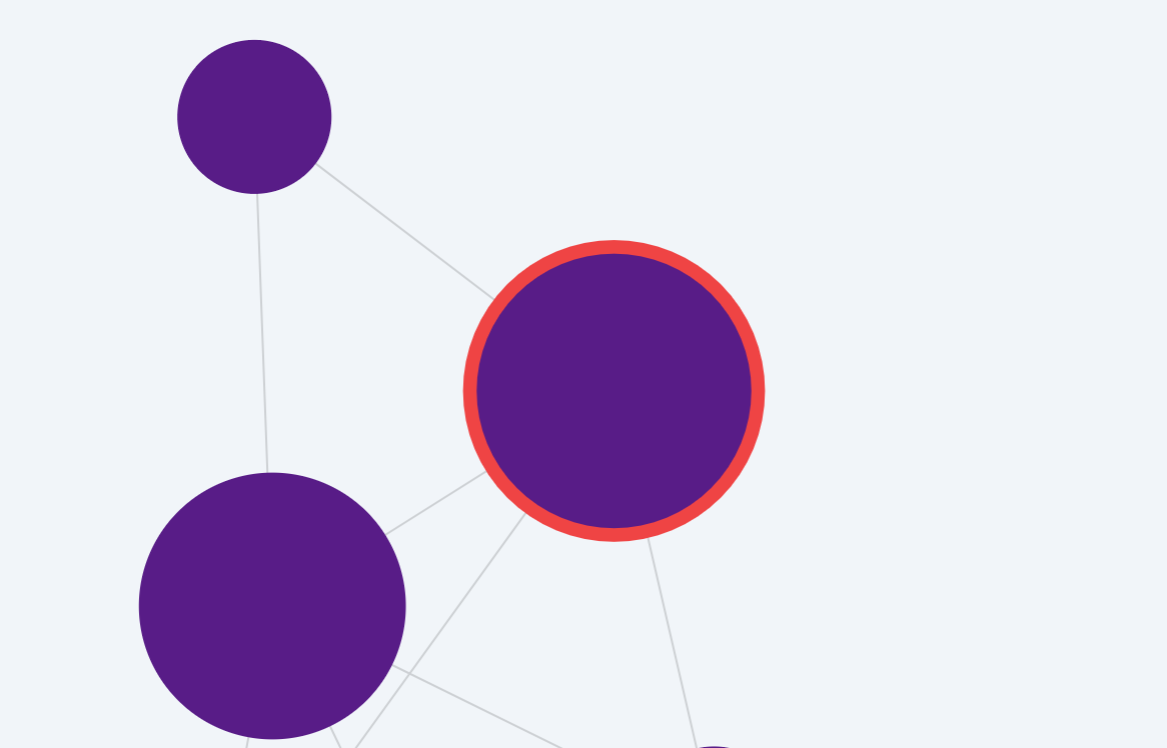
\includegraphics[width=\textwidth]{microservice_focus_graph}
  \end{subfigure}
  \hfill
  \begin{subfigure}[!htb]{0.49\textwidth}
    \centering
    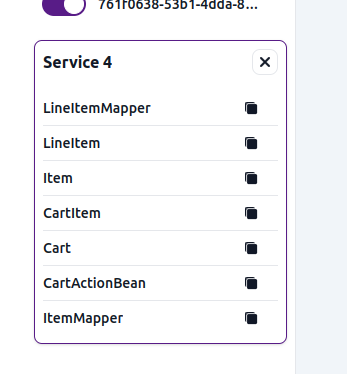
\includegraphics[width=\textwidth]{microservice_focus}
  \end{subfigure}
\end{figure*}
